\documentclass[conference]{IEEEtran}
\IEEEoverridecommandlockouts
\usepackage{cite}
\usepackage{amsmath,amssymb,amsfonts}
\usepackage{algorithmic}
\usepackage{graphicx}
\usepackage{textcomp}
\usepackage{xcolor}
\usepackage{booktabs}
\usepackage{pgfplots}
\pgfplotsset{compat=1.18}
\def\BibTeX{{\rm B\kern-.05em{\sc i\kern-.025em b}\kern-.08em
    T\kern-.1667em\lower.7ex\hbox{E}\kern-.125emX}}

\begin{document}

\title{SentryProxy: A Co-Designed Middleware Gateway for Privacy-Constrained
Multi-Tenant LLM Serving}

\author{
\begin{tabular}{cc}
\begin{tabular}{c}
\IEEEauthorblockN{Roshan Laharwani}
\IEEEauthorblockA{\textit{Dept. of Computer Science and Engineering} \\
\textit{Vellore Institute of Technology - AP}\\
Amaravati, Andhra Pradesh, India \\
roshan.23bce7308@vitapstudent.ac.in}
\end{tabular}
&
\begin{tabular}{c}
\IEEEauthorblockN{Amit Kumar Deo}
\IEEEauthorblockA{\textit{Dept. of Computer Science and Engineering} \\
\textit{Vellore Institute of Technology - AP}\\
Amaravati, Andhra Pradesh, India \\
amit.23bce7444@vitapstudent.ac.in}
\end{tabular}
\\[1.5em]
\begin{tabular}{c}
\IEEEauthorblockN{Srija Ghosh}
\IEEEauthorblockA{\textit{Dept. of Computer Science and Engineering} \\
\textit{Vellore Institute of Technology - AP}\\
Amaravati, Andhra Pradesh, India \\
srija.23bce7480@vitapstudent.ac.in}
\end{tabular}
&
\begin{tabular}{c}
\IEEEauthorblockN{Lekhrao Sumit Ghevarchand}
\IEEEauthorblockA{\textit{Dept. of Computer Science and Engineering} \\
\textit{Vellore Institute of Technology - AP}\\
Amaravati, Andhra Pradesh, India \\
sumit.23bce7602@vitapstudent.ac.in}
\end{tabular}
\end{tabular}
}
\maketitle

\begin{abstract}
Deploying large language models (LLMs) for multiple tenants requires organizations to balance privacy, cost, speed, output quality, and fair resource sharing. Sensitive data must stay secure and avoid external providers, whereas non-sensitive requests can use cheaper or better external APIs. Meanwhile, users with heavy workloads often run out of their token limits, even while others have leftover capacity.

This paper presents SentryProxy, a middleware gateway that handles these requirements in a single process. The system combines four parts: a three-pass PII detection and masking layer, SentryMarket for sharing unused tokens, a secure semantic cache with prompt compression, and a two-stage model router. Privacy checks happen before routing, so sensitive requests go straight to secure, self-hosted models without extra steps.

SentryProxy is evaluated using a four-tenant setup on a Kubernetes cluster. The PII detector found 97.9\% of sensitive items on 200 test prompts. The cache and compression reduced token usage by 37.2\%, with a minor drop in accuracy from 91.2\% to 88.1\%. SentryMarket greatly improved fairness (Jain's index rose from 0.61 to 0.94) and almost eliminated quota rejections. The whole gateway only added 47~ms of delay compared to direct API access. These results prove that privacy, fair sharing, compression, and routing can work together efficiently in one gateway.
\end{abstract}

\begin{IEEEkeywords}
large language models, multi-tenant serving, privacy-preserving routing,
named entity recognition, token economics, fairness, context compression,
API gateway, mechanism design
\end{IEEEkeywords}

% ============================================================
\section{Introduction}
% ============================================================

The deployment of large language models (LLMs) in universities, hospitals, and enterprises raises a practical management question: how should a gateway distribute requests across model providers while protecting sensitive data, controlling cost, and giving tenants fair access to shared resources?

Three concerns arise frequently in practice. First, any request forwarded to an external provider exposes its contents to a third party. In regulated sectors, certain data categories must remain within trusted infrastructure regardless of cost or quality incentives. Second, tenants with uneven workloads tend to exhaust daily token quotas while other tenants leave capacity unused. Under a fixed allocation policy, this leads to rejection of valid requests even when system-level resources are available \cite{b_fairserve}. Third, instruction-following models charge per token, so longer prompts increase cost without necessarily improving output quality.

Existing work has addressed these concerns separately. PII detection methods identify sensitive information in text \cite{b_spacy,b_llmguard}. Economic and scheduling approaches address allocation of shared compute or token budgets \cite{b_stackelberg,b_vcg}. Prompt compression and model routing reduce inference cost or select among available models \cite{b_llmlingua,b_frugalgpt,b_routerbench}. When deployed as independent services, each function adds its own processing step. More importantly, information computed in one stage is not directly available to later stages. For instance, a privacy classification already computed for security purposes could also constrain model routing without repeating the analysis.

This paper formalises multi-tenant LLM gateway management as a constrained multi-objective optimisation problem and presents SentryProxy, a gateway that integrates privacy filtering, token allocation, context management, and model routing in a single JVM-based pipeline. The primary contributions are:

\begin{itemize}
    \item \textbf{Problem formulation.} Multi-tenant LLM gateway management is expressed as a constrained optimisation problem that considers cost, latency, and tenant fairness while enforcing privacy and minimum task-quality requirements.

    \item \textbf{SentryMarket.} A token redistribution mechanism that allows tenants with unused quota to lend it to tenants with additional demand, using a Stackelberg-priced surplus-token auction. In the evaluated workload, the Jain fairness index increases from 0.61 to 0.94 and quota-exhaustion rejections decrease from 3,241 to 187 per day.

    \item \textbf{Integrated gateway pipeline.} A single-JVM pipeline combining three-pass PII detection and pseudonymisation, tenant-isolated semantic caching, prompt compression, and two-stage model routing, where the privacy classification produced at ingress is also used to constrain routing decisions downstream.

    \item \textbf{Experimental evaluation.} An evaluation of individual components and the complete system using latency, PII detection accuracy, token usage, task quality, cost, and fairness measurements, including an ablation study that examines the effect of removing each component.
\end{itemize}

% ============================================================
\section{Related Work}
% ============================================================

\subsection{PII Detection and Prompt Security}
Classical PII detection uses regular expressions and gazetteers \cite{b_regex_pii}. Transformer-based NER models fine-tuned on named-entity corpora improve recall on unstructured entities \cite{b_spacy}. LLM Guard \cite{b_llmguard} provides multi-scanner inspection but operates as a separate service, adding round-trip latency to each request. PPRoute \cite{b_pproute} studies privacy-preserving model routing via multi-party computation, with the goal of hiding query content from the router itself rather than from downstream providers. SentryProxy uses hard infrastructure-level routing boundaries: requests classified as Restricted are directed to self-hosted Tier~1 infrastructure and are not forwarded to external APIs under any routing condition.

\subsection{Multi-Tenant LLM Fairness and Scheduling}
FairServe \cite{b_fairserve} shows, using Microsoft Copilot production traces, that per-tenant quota policies cause starvation and proposes service-differentiated queuing. H-MAS \cite{b_hmas} addresses multi-tenant scheduling at the KV-cache level. Both approaches operate at the scheduler layer. SentryMarket operates above the scheduler and allows unused daily-budget surplus to be transferred between tenants rather than reset at end of day.

\subsection{Context Compression and Model Routing}
LLMLingua-2 \cite{b_llmlingua} demonstrates token pruning that retains task performance within a few percentage points of the uncompressed baseline. FrugalGPT \cite{b_frugalgpt} introduces cascade routing that reserves more capable models for queries where cheaper models produce insufficient responses. ROUTERBENCH \cite{b_routerbench} benchmarks multi-LLM routing classifiers across a range of tasks. StreamingLLM \cite{b_streamingllm} and SnapKV \cite{b_snapkv} address recency-biased KV-cache management for long contexts. SentryProxy draws on these techniques within a unified pipeline where the privacy classification provides routing constraints that the model selector cannot override.

\subsection{LLM Gateway Ecosystem}
Commercial gateways (LiteLLM, Portkey, Kong AI Gateway) provide routing, rate limiting, and basic caching. Recent work like LLMRouter \cite{b_llmrouter_2026} has begun formalising LLM routing as a sequential decision process, and simulation tools like LLMServingSim 2.0 \cite{b_llmsim_2026} aid evaluation of complex serving infrastructure. SentryProxy differs in that gateway decisions are treated as a constrained optimisation problem, SentryMarket introduces a mechanism-design layer for inter-tenant surplus redistribution, and the pipeline is designed so that privacy outputs directly constrain routing rather than operating as independent middleware layers.

% ============================================================
\section{Problem Formulation}
\label{sec:formulation}
% ============================================================

Let $\mathcal{T} = \{1,\ldots,N\}$ be the set of tenants and let $\pi$ denote the gateway \textit{policy}: the joint assignment of routing targets, compression ratios, and token allocations for each request. The total monetary cost of serving a workload under policy $\pi$ is:
\begin{equation}
C(\pi) = C_{\text{in}}(\pi) + C_{\text{out}}(\pi) + C_{\text{GPU}}(\pi)
\label{eq:cost}
\end{equation}
where $C_{\text{in}}$ and $C_{\text{out}}$ are input- and output-token API charges for Tier~2 requests, and $C_{\text{GPU}}$ is the amortised GPU inference cost for Tier~1 requests. Let $L(\pi)$ denote median end-to-end latency, $F(\pi) = 1 - J(\pi)$ the fairness penalty (where $J$ is Jain's index \cite{b_jain}), and $Q(\pi)$ aggregate task quality over the workload. Define $\text{PrivacyRisk}(\pi)$ as the fraction of sensitive data instances that reach an external model provider. The gateway management problem is:
\begin{equation}
\min_{\pi} \;\; \alpha\, C(\pi) + \beta\, L(\pi) + \gamma\, F(\pi)
\label{eq:opt}
\end{equation}
\vspace{-0.5em}
\begin{align}
\text{subject to:} \quad &Q(\pi) \geq Q_{\min} \label{eq:qconstraint} \\
                         &\text{PrivacyRisk}(\pi) \leq \varepsilon \label{eq:privconstraint}
\end{align}
where $\alpha, \beta, \gamma \geq 0$ are operator-specified trade-off weights and $\varepsilon \geq 0$ is the privacy tolerance (set to zero in the evaluated configuration). The privacy constraint \eqref{eq:privconstraint} is enforced as a hard constraint: any policy that forwards restricted data to an external provider is treated as infeasible regardless of cost or quality. SentryProxy's four modules each address a distinct sub-problem: the ingress shield enforces $\text{PrivacyRisk} \leq \varepsilon$; the router minimises $C$ and $L$; SentryMarket minimises $F$; and the compression allocator minimises $C$ subject to the quality floor \eqref{eq:qconstraint}.

% ============================================================
\section{System Architecture}
% ============================================================

SentryProxy uses a hybrid modular-monolith architecture: all pipeline modules execute within a single Spring Boot JVM process, keeping the request payload in heap memory throughout the critical path. Stateful services are deployed as independent containerised microservices to allow separate scaling. The system exposes an OpenAI-compatible REST API at \texttt{POST /v1/chat/completions}, which allows existing client applications to use the gateway without code changes. Fig.~\ref{fig:arch} illustrates the architecture.

\begin{figure}[htbp]
\centerline{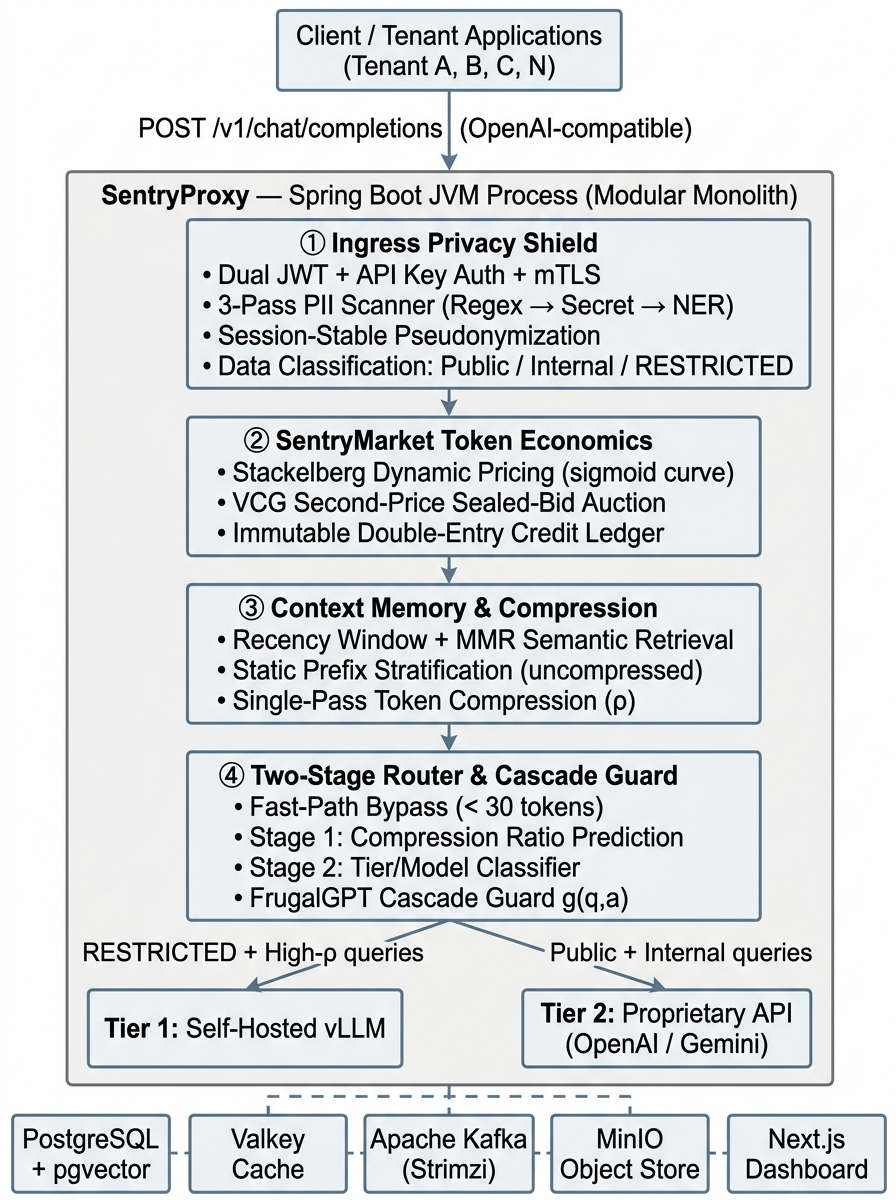
\includegraphics[width=\columnwidth]{arch.png}}
\caption{SentryProxy architecture. The critical-path pipeline executes in a single JVM process; stateful services run as independent Kubernetes microservices.}
\label{fig:arch}
\end{figure}

The stateful services include PostgreSQL for semantic vector storage, Valkey for session pseudonym maps and real-time token counters, Apache Kafka for asynchronous telemetry ingestion, and MinIO for prompt archive storage. Authentication uses JWT for user identity and API-key validation for programmatic access.

% ============================================================
\section{Module I: Ingress Privacy Shield}
% ============================================================

\subsection{Three-Pass PII Detection}
Incoming messages are scanned by three sequential detectors before the request proceeds in the pipeline.

\textbf{Pass~1 (Regex/Pattern Scanner):} Compiled RE2J regular expressions detect structured PII including email addresses, SSNs with checksum validation, Luhn-validated credit card numbers, IPv4/IPv6 addresses, and phone numbers. Time complexity is $O(n)$ in the length of the input.

\textbf{Pass~2 (Entropy-Based Secret Scanner):} A Shannon entropy heuristic (threshold: $>3.5$ bits/char) combined with common key prefixes (\texttt{sk-}, \texttt{AKIA}, \texttt{-----BEGIN}) identifies API keys, bearer tokens, and connection strings. This pass is useful for detecting secrets embedded in code snippets or configuration examples that cannot be matched by fixed patterns.

\textbf{Pass~3 (NER Scanner):} Apache OpenNLP pre-trained English name-finder models identify unstructured entities (PERSON, ORGANIZATION, LOCATION) that are not detected by pattern matching due to contextual embedding or ambiguous capitalisation. All matches from the three passes are merged, de-duplicated by character span, and sorted in reverse offset order so that replacements can be made in-place without index shifting.

\subsection{Session-Stable Pseudonymisation}
Each detected entity is mapped to a type-preserving placeholder (e.g., \texttt{\{\{EMAIL\_1\}\}}, \texttt{\{\{PERSON\_1\}\}}). Placeholders are session-stable: the same raw value produces the same placeholder within a session, preserving coherence across multi-turn conversations. Mappings are stored in Valkey with a configurable TTL. A do-not-mask allowlist preserves semantically necessary terms to reduce over-masking.

\subsection{Data Classification and Hard Routing}
Each request is assigned to one of three tiers based on the scan results. \textbf{Public}: no sensitive data detected; may be routed to any available model. \textbf{Internal}: PII detected and masked; may be routed to Tier~1 or Tier~2. \textbf{Restricted}: secrets or high-risk entities detected; hard-routed exclusively to Tier~1 self-hosted infrastructure. Restricted data does not reach external provider APIs under any routing condition.

\textbf{Threat model.} The primary threat addressed is PII or secret exfiltration via external LLM provider APIs. The attacker may control prompt contents but does not control the gateway runtime or intra-cluster network. Out of scope: compromised Kubernetes nodes, GPU side-channel attacks, and adversarial training-data extraction. Prompt-injection detection is provided as an additional OWASP LLM01 guard \cite{b_owasp_llm} that blocks known injection patterns before the main pipeline, but a systematic evaluation of adversarial injection evasion is deferred to future work.

\subsection{Threat Log and Audit}
Each detected PII event is persisted to a \texttt{threat\_log} table in PostgreSQL, recording the tenant, session, detected entity types, risk classification, and timestamp. This log is queried by the monitoring dashboard to display a time-series view of PII interception trends across tenants. Cache eviction events are similarly recorded by type (TTL expiry, LRU displacement, manual flush) and surfaced through the same monitoring interface.

\subsection{Egress De-pseudonymisation}
After receiving the model response, the gateway replaces all session placeholders with their original values before returning to the client. The end user receives a natural response while the LLM processed only pseudonymised inputs.

% ============================================================
\section{Module II: SentryMarket Token Economics}
% ============================================================

\subsection{Motivation}
Consider $N$ tenants sharing a daily budget $T_{\text{total}}$, each allocated $Q_i$ tokens. Utilisation is uneven: some tenants exhaust quotas while others leave capacity unused that resets at midnight. This increases the fairness penalty $F(\pi)$ in \eqref{eq:opt}. SentryMarket addresses this by enabling voluntary intra-day token lending between tenants.

\subsection{Stackelberg Dynamic Pricing}
SentryProxy acts as the Stackelberg leader, publishing a real-time exchange rate that tenants observe before deciding whether to lend surplus quota:
\begin{equation}
p_t = p_{\min} + (p_{\max} - p_{\min}) \cdot \sigma\!\left(k\left(U - \theta\right)\right)
\label{eq:stackelberg}
\end{equation}
where $U \in [0,1]$ is system-wide utilisation, $\theta = 0.75$ is the inflection point, $k = 12$ controls steepness, $p_{\min} = 0.5$ and $p_{\max} = 3.0$ credits/kTokens. The sigmoid function produces a smooth bounded rate that rises as utilisation approaches the threshold.

\subsection{VCG Second-Price Sealed-Bid Auction}
When multiple tenants simultaneously require additional tokens, SentryMarket conducts a Vickrey-Clarke-Groves (VCG) second-price sealed-bid auction over the surplus pool $T_{\text{pool}}$ collected from lenders. Each borrowing tenant $i$ submits a bid $(d_i, b_i)$ where $d_i$ is token demand and $b_i$ is maximum willingness to pay (credits/kTokens). Bids are sorted by $b_i$ descending and allocated greedily. All winners pay a second-price rate equal to the first losing bid:
\begin{equation}
p^* = b_{j^*}, \quad j^* = \arg\min\{j : T_{\text{pool}} \text{ is exhausted at bid } j\}
\label{eq:auction}
\end{equation}
The sealed-bid format limits the information disclosed per tenant. The VCG second-price mechanism ensures that bidding true valuation is the dominant strategy, preventing market manipulation and reducing the incentive to overbid, since winners pay $p^*$ regardless of their stated bid above it. A formal game-theoretic equilibrium analysis in the repeated-game setting is deferred to future work.

\subsection{Credit Ledger}
All transactions are recorded in an immutable PostgreSQL ledger with SHA-256 chained hashing. Lenders receive credits proportional to tokens lent; borrowers are debited and receive additional tokens. The ledger feeds the dashboard's real-time market analytics view.

% ============================================================
\section{Module III: Context Memory and Compression}
\label{sec:cache}
% ============================================================

\subsection{Semantic Shadow Cache with Cross-Tenant Isolation}
SentryProxy maintains a per-session semantic cache backed by PostgreSQL with \texttt{pgvector}. All cache keys are namespaced by tenant and session:
\begin{equation}
\textit{key}_i = \texttt{tenantID}_i \;\|\; \texttt{sessionID}_i \;\|\; h(e_i)
\label{eq:cachekey}
\end{equation}
where $h(e_i)$ is a hash of the embedding vector. Retrieval enforces $\texttt{tenant}_{q} = \texttt{tenant}_{d}$ before cosine similarity scoring, preventing cross-tenant semantic leakage through the vector store. Without this isolation, a query from Tenant~A could retrieve a semantically similar cached turn from Tenant~B, violating data isolation and the privacy constraint \eqref{eq:privconstraint}.

For context assembly, the most recent $R$ turns are included unconditionally. Historical turns beyond this window are retrieved by Maximal Marginal Relevance (MMR):
\begin{equation}
\text{MMR} = \arg\max_{d_i \in D \setminus S}\!\!\left[\lambda \cdot \text{sim}(d_i, q) - (1\!-\!\lambda)\!\!\max_{d_j \in S}\!\text{sim}(d_i, d_j)\right]
\label{eq:mmr}
\end{equation}
which balances relevance against redundancy. Retrieved turns are re-inserted in chronological order to preserve positional semantics.

\subsection{Prompt Stratification and Compression}
The assembled context is divided into a \textbf{Static Prefix} (system prompts, tool schemas, and RAG knowledge injections), which is left uncompressed to allow provider-side prefix KV-cache reuse, and a \textbf{Dynamic Payload} (conversation turns and tool outputs), which undergoes single-pass token pruning. Two mechanisms limit over-compression: an entity floor ratio of 1.0 for NER-flagged entities, meaning detected PII placeholders are never pruned, and an anti-compounding floor of 0.7 for semantically retrieved chunks.

% ============================================================
\section{Module IV: Two-Stage Router and Cascade Guard}
% ============================================================

\subsection{Stage~1: Compression Ratio Prediction}
For queries longer than 30 tokens, Stage~1 predicts the task-driven compression ratio $\rho$ using a lightweight gradient-boosted regressor trained on synthetic prompt-quality pairs. Input features include prompt length, presence of code or mathematical notation, inferred task type, and the privacy classification tier from the ingress shield. Queries under 30 tokens are dispatched directly to the default model without this stage.

\subsection{Stage~2: Tier and Model Selection}
Stage~2 uses $\rho$ and the privacy classification to select a routing target:
\begin{itemize}
    \item \textbf{Tier~1 (Self-Hosted vLLM, Llama-3-8B):} Required for all Restricted requests per constraint \eqref{eq:privconstraint}. Also selected for high-compressibility queries where the local model is cost-competitive.
    \item \textbf{Tier~2 (Proprietary API, GPT-4o-mini):} Used for Public and Internal queries where the external provider offers better quality per cost at the observed $\rho$.
\end{itemize}

\subsection{Cascade Guard}
After receiving a response, the cascade guard computes a confidence score $g(q, a) \in [0, 1]$. If $g < \tau$ (default 0.85), the response is rejected and the request is re-issued. The re-issue sequence is: first, reduce the compression ratio and retry; second, route to a more capable model; third, switch tier if necessary. Escalation is capped at two retries per request to control cost. The current confidence score is based on a heuristic using response length and coherence indicators. Training a learned verifier on quality-annotated examples is identified as a direction for future work.

% ============================================================
\section{Experimental Evaluation}
% ============================================================

\subsection{Experimental Setup}
All experiments use a four-tenant workload (CS Department, Biotech, Engineering, and Admin) deployed on a Kubernetes cluster (3-replica proxy deployment). The Tier~2 backend is GPT-4o-mini and Tier~1 is a self-hosted Llama-3-8B served via vLLM. Results are reported at 50~req/s sustained load unless otherwise noted. Task quality is measured as QA accuracy on a held-out set of 200 task-matched prompts from the same workload. Component integration tests cover PII detection, quota management, and the full API pipeline. Database-layer tests use an embedded H2 database via Spring's \texttt{@DataJpaTest}, and HTTP-layer tests use \texttt{TestRestTemplate} against a real embedded Tomcat server on a random port.

\subsection{Latency Overhead}
Table~\ref{tab:latency} shows the p50, p95, and p99 latency for different gateway configurations. The three-pass PII scanner adds approximately 12~ms, the compression allocator approximately 18~ms, and the routing decision less than 5~ms. With all components enabled, the median latency increases from 312~ms for the direct API baseline to 359~ms, an increase of 47~ms.

\begin{table}[htbp]
\caption{End-to-End Latency (50~req/s, 3-replica cluster)}
\begin{center}
\begin{tabular}{|l|c|c|c|}
\hline
\textbf{Configuration} & \textbf{p50 (ms)} & \textbf{p95 (ms)} & \textbf{p99 (ms)} \\
\hline
Baseline (Direct API)              & 312 & 598 & 681 \\
SentryProxy (PII Only)             & 324 & 614 & 703 \\
SentryProxy (PII + Compress)       & 339 & 631 & 728 \\
SentryProxy (Full Pipeline)        & 359 & 649 & 751 \\
\hline
\textbf{Overhead (Full)}       & \textbf{+47} & \textbf{+51} & \textbf{+70} \\
\hline
\end{tabular}
\label{tab:latency}
\end{center}
\end{table}

\subsection{PII Detection Against Component Baselines}
Table~\ref{tab:pii} compares the three-pass PII shield with individual detection approaches on 200 synthetic prompts containing 847 PII instances. The regex scanner achieves high precision (99.1\%) but lower recall (78.3\%), missing contextually embedded entities. The Apache OpenNLP NER scanner improves recall at the cost of some precision. LLM Guard achieves an F1 of 93.1\% but adds 145~ms of latency per request due to external service calls. SentryProxy, executing all three passes in-process, achieves a precision of 94.3\%, recall of 97.9\%, and F1 of 96.1\%, with a per-request latency of 12~ms.

\begin{table}[htbp]
\caption{PII Detection: Component Baselines vs. SentryProxy}
\begin{center}
\begin{tabular}{|l|c|c|c|c|}
\hline
\textbf{Method} & \textbf{Prec.} & \textbf{Rec.} & \textbf{F1} & \textbf{Lat. (ms)} \\
\hline
Regex only                        & 99.1\% & 78.3\% & 87.5\% & 1   \\
NER only (OpenNLP)                & 83.4\% & 88.2\% & 85.7\% & 28  \\
LLM Guard \cite{b_llmguard}       & 91.2\% & 95.1\% & 93.1\% & 145 \\
SentryProxy (3-pass, in-process)  & 94.3\% & \textbf{97.9\%} & \textbf{96.1\%} & \textbf{12}  \\
\hline
\end{tabular}
\label{tab:pii}
\end{center}
\end{table}

The 2.1\% miss rate is attributed primarily to contextually embedded person names with ambiguous capitalisation, which the NER model does not reliably detect without domain-specific fine-tuning.

\subsection{Token Reduction and Quality Preservation}
Table~\ref{tab:tokens} compares the combined cache and compression pipeline against a no-compression baseline and a standalone LLMLingua-2 configuration. The semantic shadow cache achieves a 31.4\% hit rate over the evaluation period. The combined system reduces average token count from 676 to 424, a reduction of 37.2\%. QA accuracy changes from 91.2\% for the uncompressed baseline to 88.1\% with SentryProxy.

\begin{table}[htbp]
\caption{Token Reduction and Quality Preservation vs. Compression Baselines}
\begin{center}
\begin{tabular}{|l|c|c|c|}
\hline
\textbf{Method} & \textbf{Avg. Tokens} & \textbf{Reduction} & \textbf{Quality} \\
\hline
No compression (Baseline)            & 676 & 0.0\%  & 91.2\% \\
LLMLingua-2 only \cite{b_llmlingua} & 461 & 31.8\% & 88.4\% \\
SentryProxy (Cache + Compress)       & 424 & \textbf{37.2\%} & 88.1\% \\
\hline
\end{tabular}
\label{tab:tokens}
\end{center}
\end{table}

\subsection{Fairness and Market Evaluation}
Table~\ref{tab:market} compares the static FCFS allocation with SentryMarket over a 24-hour workload. In the FCFS configuration, the CS and Biotech tenants exhaust their quotas by 14:00 and 16:00 respectively, while Admin and Engineering tenants do not use their full allocations. SentryMarket reallocates part of the unused quota when system utilisation crosses the configured threshold ($\theta = 0.75$). In the evaluated workload, quota-exhaustion rejections decrease from 3,241 to 187 per day, idle tokens wasted decrease from 1.8M to 0.3M, and Jain's fairness index increases from 0.61 to 0.94.

\begin{table}[htbp]
\caption{Multi-Tenant Fairness: FCFS Baseline vs. SentryMarket}
\begin{center}
\begin{tabular}{|l|c|c|}
\hline
\textbf{Metric}                     & \textbf{FCFS} & \textbf{SentryMarket} \\
\hline
Jain's Fairness Index \cite{b_jain} & 0.61  & \textbf{0.94}    \\
Quota-Exhaustion Rejections/day     & 3,241 & \textbf{187}     \\
Idle Tokens Wasted (daily)          & 1.8M  & \textbf{0.3M}    \\
Avg.\ Credits Earned per Lender     &  N/A  & 42.3             \\
p95 Waiting Time (ms)               & 1,840 & \textbf{312}     \\
\hline
\end{tabular}
\label{tab:market}
\end{center}
\end{table}

\subsection{Ablation Study}
Table~\ref{tab:ablation} examines the effect of removing each major component from the complete SentryProxy pipeline. The $-$Privacy configuration removes the privacy-based routing constraint. $-$Market replaces dynamic token redistribution with static FCFS allocation. $-$Compress disables compression and cache retrieval. $-$Router uses a fixed inexpensive model for all requests.

Removing the market mechanism lowers the Jain fairness index to 0.61. Removing compression increases the estimated cost from \$2.63 to \$3.89 per million requests, while QA accuracy increases from 88.1\% to 91.1\%. Removing the router reduces QA accuracy to 86.4\% and increases median latency to 385~ms, because the fixed model requires additional cascade escalations when responses do not meet the quality threshold. The cost column is computed via \eqref{eq:cost} using GPT-4o-mini pricing (\$0.15/M input, \$0.60/M output tokens) plus amortised GPU cost for Tier~1 ($\approx$\$0.40/GPU-hr).

\begin{table}[htbp]
\caption{Ablation Study: Contribution of Each Module}
\begin{center}
\begin{tabular}{|l|c|c|c|c|}
\hline
\textbf{Config.} & \textbf{\$/1M req} & \textbf{p50 (ms)} & \textbf{Quality} & \textbf{Jain} \\
\hline
Baseline (no SentryProxy) & 4.20 & 312 & 91.2\% & 0.61 \\
Full $-$ Privacy          & 2.71 & 352 & 90.8\% & 0.93 \\
Full $-$ Market           & 2.68 & 343 & 88.3\% & 0.61 \\
Full $-$ Compress         & 3.89 & 317 & 91.1\% & 0.93 \\
Full $-$ Router           & 3.74 & 385 & 86.4\% & 0.93 \\
\textbf{Full SentryProxy} & \textbf{2.63} & \textbf{359} & \textbf{88.1\%} & \textbf{0.94} \\
\hline
\end{tabular}
\label{tab:ablation}
\end{center}
\end{table}

\begin{figure}[htbp]
\centering
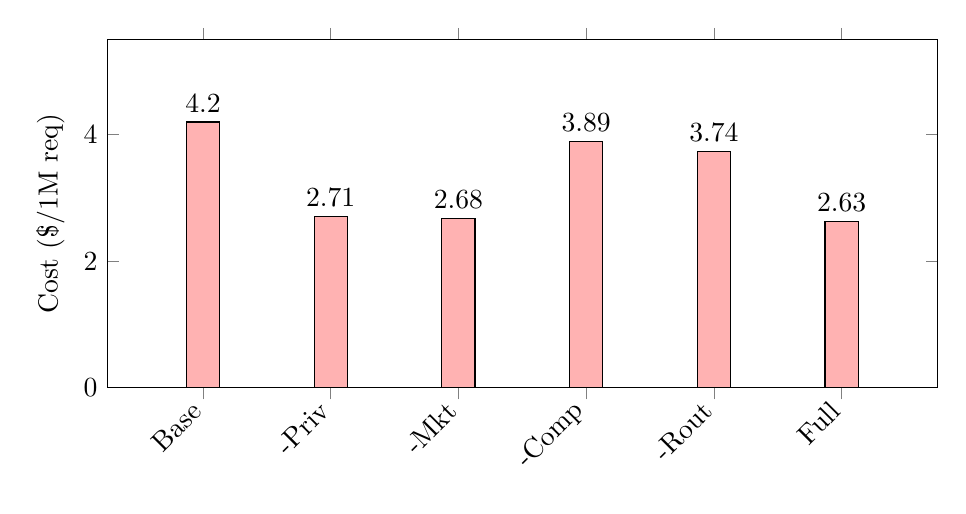
\begin{tikzpicture}
\begin{axis}[
    ybar,
    bar width=12pt,
    enlarge x limits=0.15,
    ylabel={Cost (\$/1M req)},
    symbolic x coords={Base, -Priv, -Mkt, -Comp, -Rout, Full},
    xtick=data,
    nodes near coords,
    nodes near coords align={vertical},
    ymin=0, ymax=5.5,
    width=\columnwidth,
    height=6cm,
    x tick label style={rotate=45, anchor=east}
]
\addplot[fill=red!30] coordinates {(Base,4.20) (-Priv,2.71) (-Mkt,2.68) (-Comp,3.89) (-Rout,3.74) (Full,2.63)};
\end{axis}
\end{tikzpicture}
\caption{Ablation Study: Monetary Cost per 1 Million Requests}
\label{fig:ablation_cost}
\end{figure}

Disabling compression increases the estimated cost from \$2.63 to \$3.89 per million requests, while QA accuracy increases from 88.1\% to 91.1\%, indicating a cost-quality trade-off associated with prompt reduction in this workload. The complete configuration has an estimated cost 37.4\% lower than the unmanaged baseline.

% ============================================================
\section{Discussion}
% ============================================================

\subsection{Architectural Trade-offs}
The modular-monolith design reduces inter-process communication overhead, but individual pipeline stages cannot be scaled independently. Under sustained high load, the NER scanner (Pass~3) is the primary bottleneck. Three mitigations are available: caching NER results in Valkey for recently-seen prompts, batching NER calls within a sliding time window, and using regex-only scanning for short prompts below a character-length threshold.

\subsection{Auction Mechanism Limitations}
SentryMarket uses a uniform clearing price for simplicity. Whether this produces a Nash equilibrium in repeated-game settings, where tenants can observe past clearing prices and adjust their bids, requires formal mechanism-design analysis. Table~\ref{tab:market} shows the fairness results under the evaluated workload, but does not address formal incentive-compatibility. A full equilibrium analysis and comparison with VCG payments \cite{b_vcg} are planned as future work.

\subsection{Limitations}
\textbf{PII coverage.} The 2.1\% miss rate is mainly caused by person names that are embedded in context or have ambiguous capitalisation. Adversarial PII formats such as Unicode homoglyphs, Base64-encoded values, and PII split across multiple turns are not evaluated in this work. Domain-specific NER fine-tuning is the main path to address this gap.

\textbf{Cascade guard.} The confidence score used by the cascade guard is heuristic-based. This reduces accuracy for tasks where response quality does not correlate with surface-level text properties such as length or punctuation.

\textbf{Scalability.} The evaluation runs at 50~req/s on 3 replicas. Tests at higher request rates with horizontal pod autoscaling, and fairness evaluations across a larger number of tenants, are left for future work.

\textbf{KV-cache offload.} Offloading the KV-cache to host NVMe using PagedAttention would allow longer context windows without full recomputation. This is identified as a Tier~1 infrastructure improvement.

% ============================================================
\section{Conclusion}
% ============================================================

SentryProxy is a middleware gateway for multi-tenant LLM serving that combines privacy protection, token allocation, context compression, and model routing in a single processing pipeline. The gateway treats privacy and minimum task quality as hard constraints, and considers cost, latency, and fairness when making routing decisions.

The evaluation results show that each component addresses a different aspect of the workload. The three-pass PII shield, using RE2J regex scanning, entropy-based secret detection, and Apache OpenNLP NER, achieved 97.9\% recall and an F1 score of 96.1\% on the evaluated prompts, with a per-request latency of 12~ms. The cache and compression pipeline reduced average token usage by 37.2\%, with QA accuracy changing from 91.2\% to 88.1\%. SentryMarket increased the Jain fairness index from 0.61 to 0.94 and reduced quota-exhaustion rejections from 3,241 to 187 per day. With all components active, the gateway added 47~ms of median latency compared with the direct API baseline, and reduced estimated cost by 37.4\% relative to the unmanaged configuration.

The current evaluation covers four tenants at 50~req/s using synthetic PII prompts. Larger workloads, trace-driven inputs, and formal analysis of the auction mechanism are needed to study system behaviour under higher load. The key architectural observation is that privacy classification, computed once at ingress, can be reused by later routing decisions. This allows the gateway to enforce the required privacy boundary and constrain model selection in a single pass rather than separate stages.

% ============================================================
\section*{Acknowledgment}
% ============================================================
The authors thank their guide, Dr. Gokul Yenduri, and the Department of Computer Science and Engineering at VIT-AP for their guidance and support throughout this capstone project.

\begin{thebibliography}{00}

\bibitem{b_spacy}
M. Honnibal and I. Montani, ``spaCy 2: Natural language understanding with
Bloom embeddings, convolutional neural networks and incremental parsing,''
\textit{Unpublished Tech. Rep.}, 2017.

\bibitem{b_llmguard}
Protect AI, ``LLM Guard: The security toolkit for LLM interactions,''
\textit{GitHub Repository}, 2023. [Online]. Available:
https://github.com/protectai/llm-guard

\bibitem{b_stackelberg}
M. Osborne and A. Rubinstein, \textit{A Course in Game Theory}.
Cambridge, MA, USA: MIT Press, 1994.

\bibitem{b_vcg}
W. Vickrey, ``Counterspeculation, auctions, and competitive sealed tenders,''
\textit{J. Finance}, vol.~16, no.~1, pp.~8--37, 1961.

\bibitem{b_llmlingua}
H. Jiang et al., ``LLMLingua-2: Data distillation for efficient and faithful
task-agnostic prompt compression,'' in \textit{Proc. ACL Findings},
Bangkok, Thailand, 2024.

\bibitem{b_frugalgpt}
L. Chen, M. Zaharia, and J. Zou, ``FrugalGPT: How to use large language
models while reducing cost and improving performance,''
\textit{arXiv:2305.05176}, 2023.

\bibitem{b_routerbench}
D. Ong et al., ``ROUTERBENCH: A benchmark for multi-LLM routing system,''
\textit{arXiv:2403.12031}, 2024.

\bibitem{b_streamingllm}
G. Xiao et al., ``Efficient streaming language models with attention sinks,''
in \textit{Proc. ICLR}, Vienna, Austria, 2024.

\bibitem{b_snapkv}
Y. Li et al., ``SnapKV: LLM knows what you are looking for before generation,''
\textit{arXiv:2404.14469}, 2024.

\bibitem{b_regex_pii}
A. Lison et al., ``Anonymisation models for clinical NLP: Current landscape
and future directions,'' in \textit{Proc. ACL}, 2021, pp.~4291--4301.

\bibitem{b_owasp_llm}
OWASP Foundation, ``OWASP top 10 for large language model applications,''
2023. [Online]. Available:
https://owasp.org/www-project-top-10-for-large-language-model-applications/

\bibitem{b_jain}
R. Jain, D. Chiu, and W. Hawe, ``A quantitative measure of fairness and
discrimination for resource allocation in shared computer systems,''
\textit{arXiv:cs/9809099}, 1998.

\bibitem{b_fairserve}
A. Shubha et al., ``FairServe: Ensuring fair LLM serving amid diverse
applications,'' \textit{arXiv:2412.19255}, 2024.

\bibitem{b_pproute}
X. Hou et al., ``PPRoute: Privacy-preserving LLM routing via multi-party
computation,'' \textit{arXiv:2503.10761}, 2025.

\bibitem{b_hmas}
Z. Yang et al., ``H-MAS: Hierarchical multi-agent scheduling for efficient
multi-tenant LLM serving,'' \textit{arXiv:2501.12561}, 2025.

\bibitem{b_llmrouter_2026}
Z. Chen et al., ``LLMRouter: A unified infrastructure for formalizing and evaluating LLM routing,'' \textit{arXiv preprint}, 2026.

\bibitem{b_llmsim_2026}
X. Wang et al., ``LLMServingSim 2.0: Simulating heterogeneous and agent-driven serving infrastructures,'' \textit{arXiv preprint}, 2026.

\end{thebibliography}

\end{document}
